\documentclass[12pt]{article}
\usepackage{geometry}                % See geometry.pdf to learn the layout options. There are lots.
\geometry{letterpaper}                   % ... or a4paper or a5paper or ... 
%\geometry{landscape}                % Activate for for rotated page geometry
%\usepackage[parfill]{parskip}    % Activate to begin paragraphs with an empty line rather than an indent
\usepackage{graphicx}
\usepackage{amssymb}
\usepackage{subfig}
\usepackage{pstricks,pst-node,pst-tree}



\title{Analysis of loadings}
\author{Wesley Brooks}
\date{}                                           % Activate to display a given date or no date

\usepackage{Sweave}
\begin{document}
\setkeys{Gin}{width=0.9\textwidth}    %make figures a bit wider than the Sweave default.
\maketitle

First, we'll read the data files.\\



Next, divide the events into three classes: one class for events that occured with snowmelt, one class for events that occured after the spring's last snowmelt but before mid-May (defined here as Julian date 135), and one class for events that occured after julian 135 and before the first snowmelt of the next winter.

We also will look at dividing the data into just two groups: one that is snow-influenced and one that is not. "Not snow-influenced" just combines event classes two and three.\\





Produce plots of the proportion of the suspended solids and phosphorus (both total loading and stormflow loading) that is contributed by each class of event at each stream site:\\



\begin{figure}
    \begin{center}
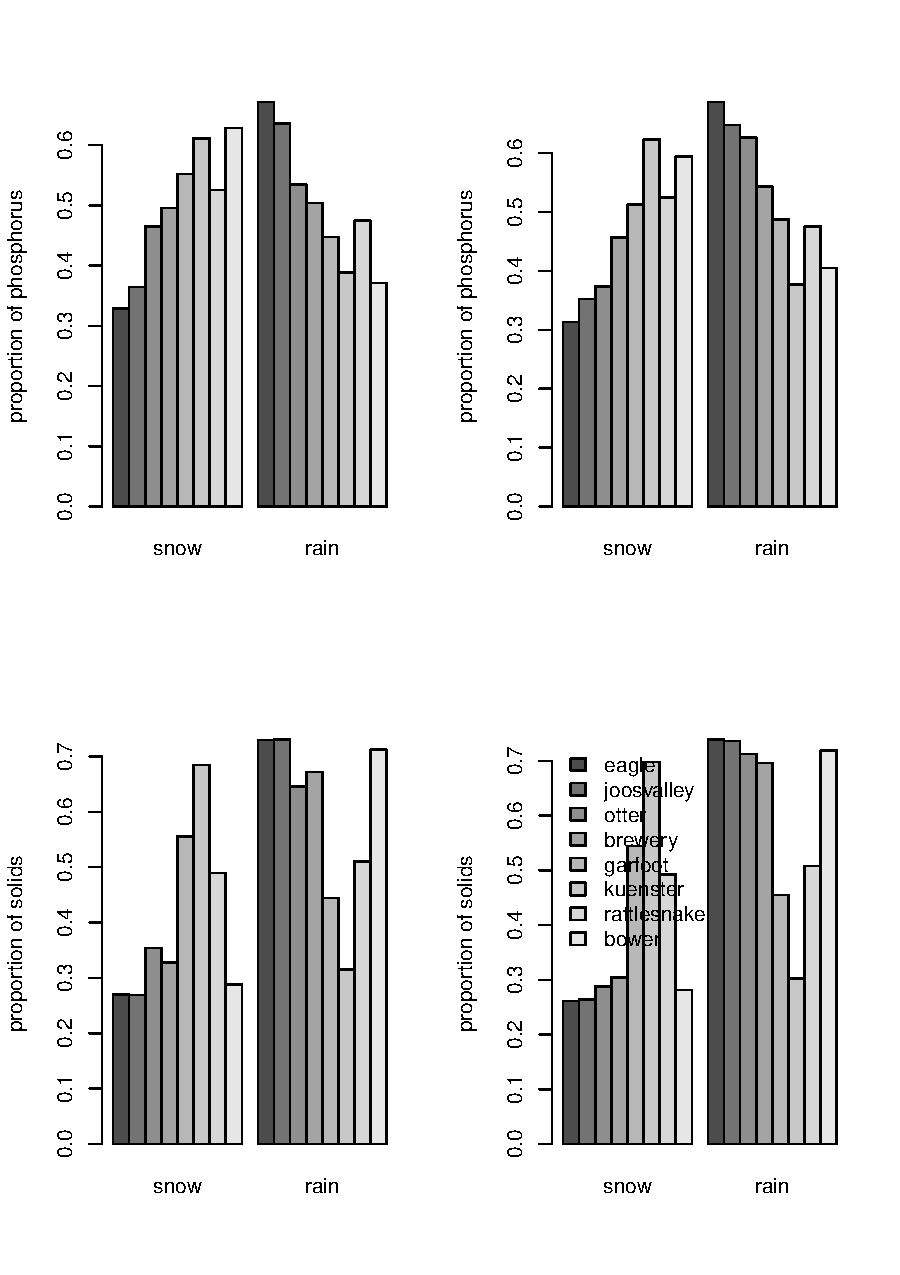
\includegraphics{loadings-fig2}
    \end{center}
    \caption{Cumulative storm loadings at the three creeks.\label{bars}}
\end{figure}



Now let's do the same between the snow and no-snow events:\\





\begin{figure}
    \begin{center}
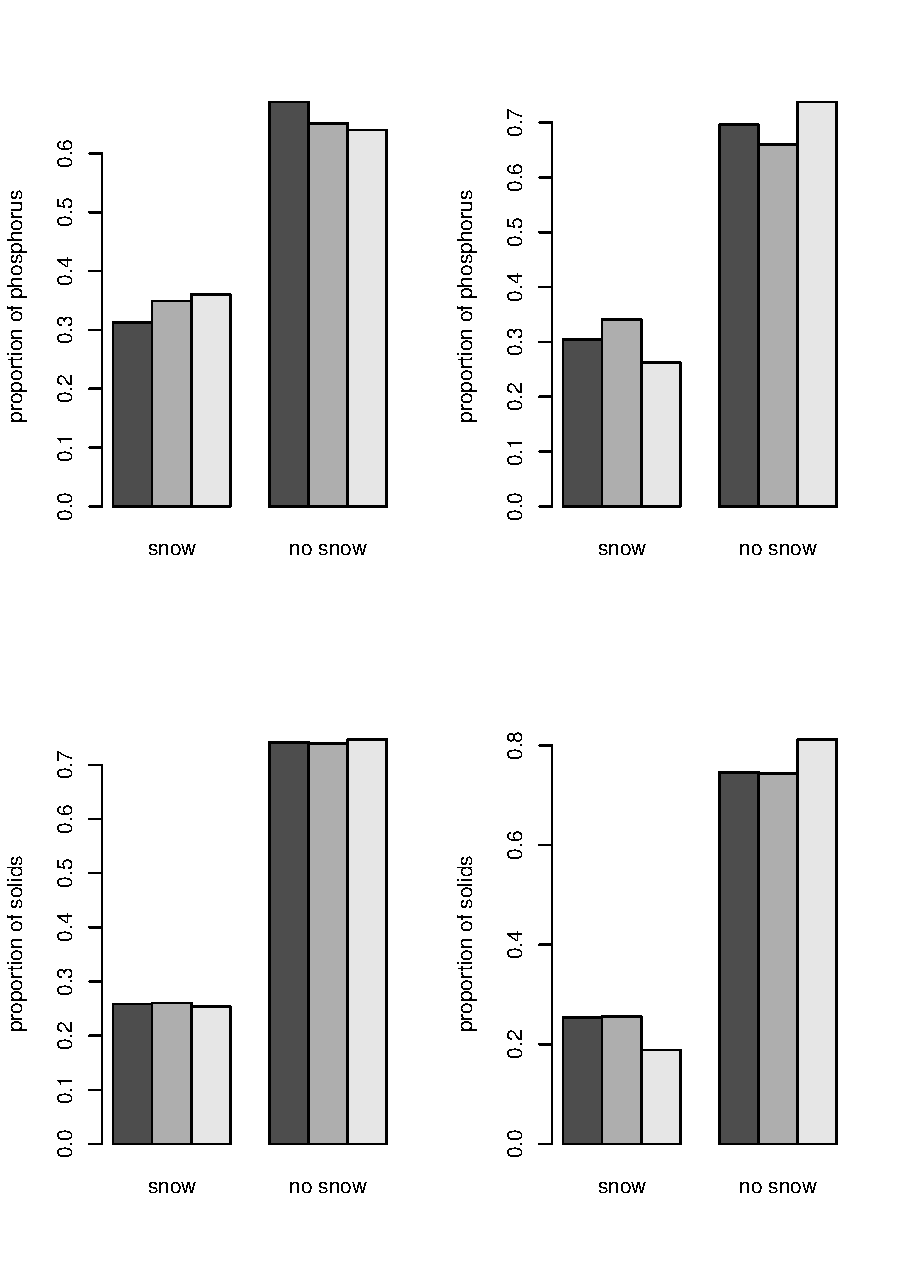
\includegraphics{loadings-fig3}
    \end{center}
    \caption{Cumulative storm loadings at the three creeks.\label{bars2}}
\end{figure}



Figure out what proportion of total storm loading is contributed by the top 10\% of storms:\\


The top 10\% of storms contributed 92.4\% of the storm loading at Eagle Creek, 81.3\% of the storm loading at Otter Creek, and 95.8\% of the storm loading at Joos Valley Creek.\\


\begin{figure}
    \begin{center}
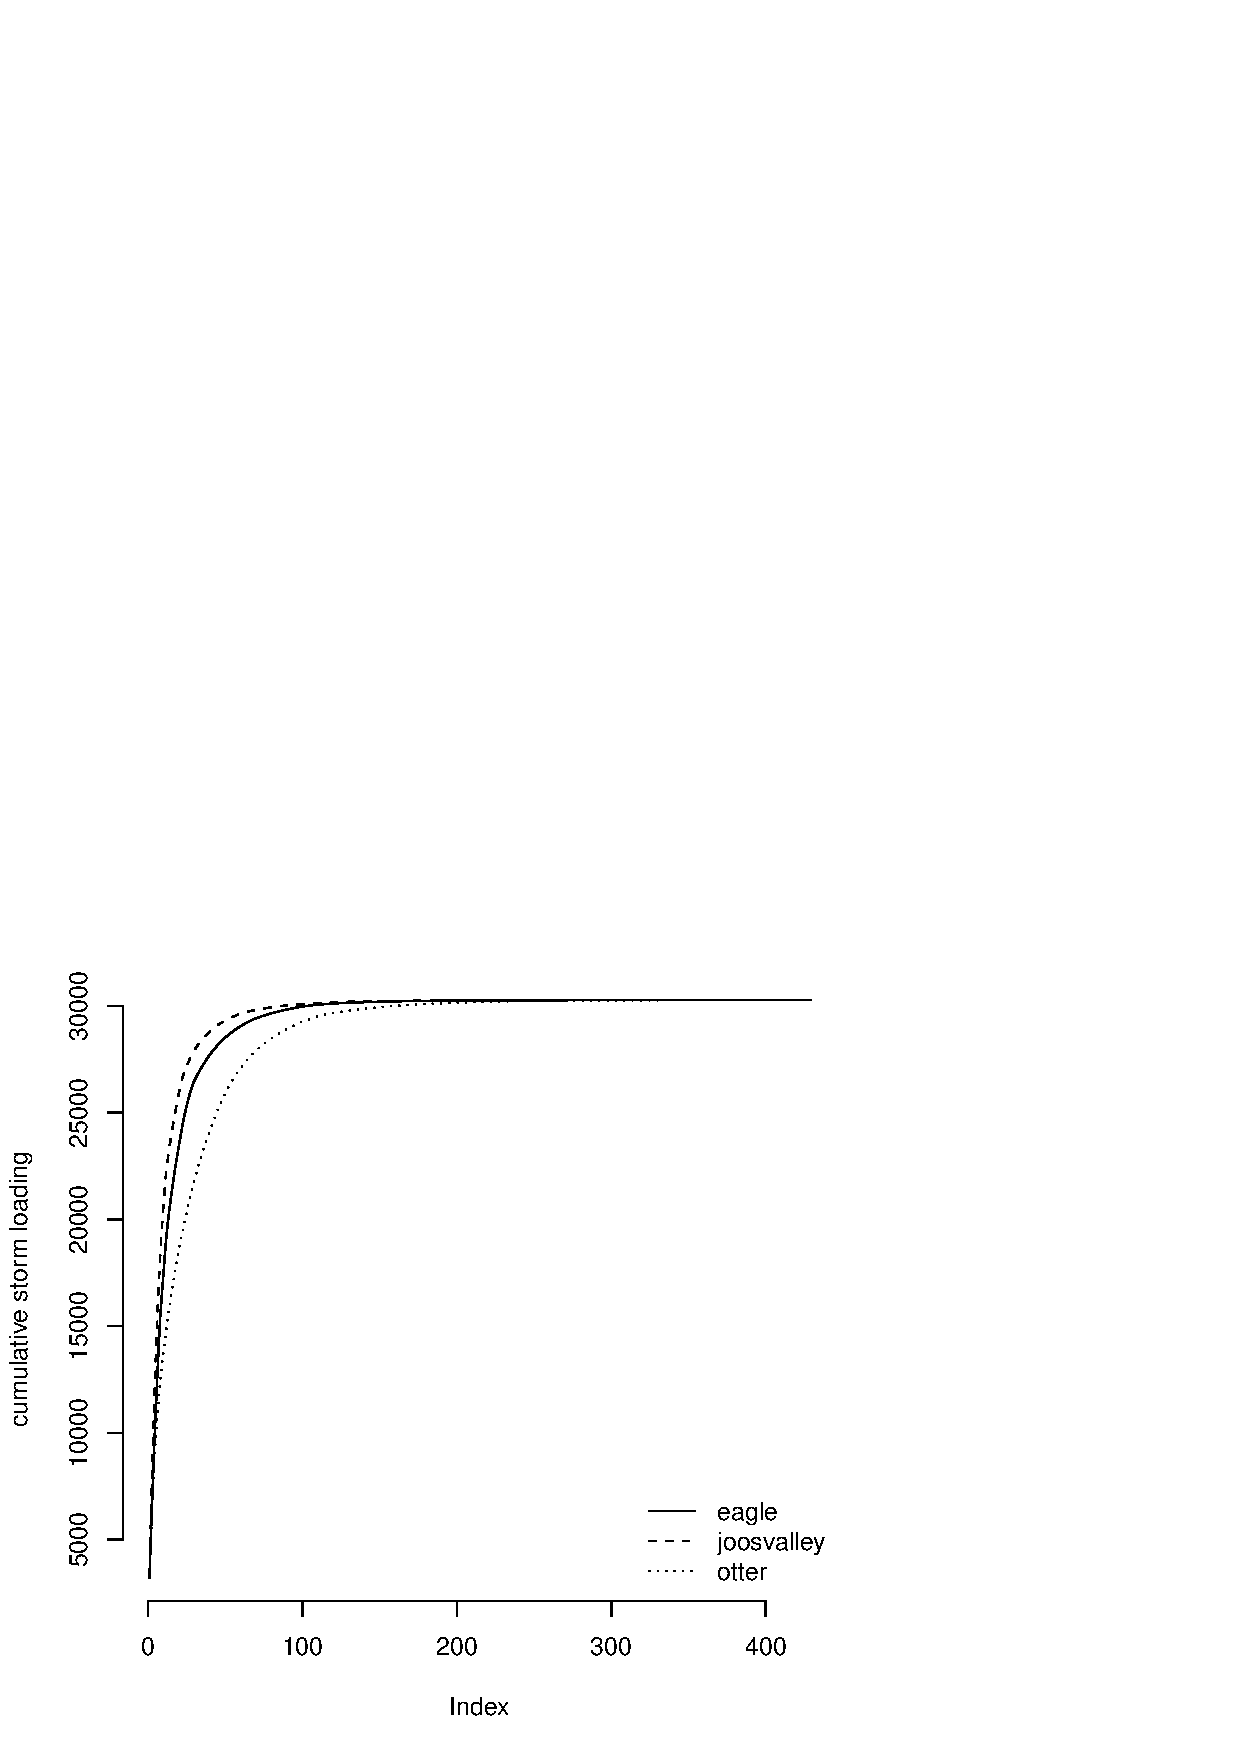
\includegraphics{loadings-figure1}
    \end{center}
    \caption{Cumulative storm loadings at the three creeks.\label{cdf}}
\end{figure}



 %\begin{landscape}
 \begin{center}
\psset{linecolor=black,tnsep=2pt,tnheight=0cm,treesep=.3cm,levelsep=40pt,radius=10pt}
%     \def\psedge#1#2{\ncangle{#2}{#1}}
%     \pstree[treemode=R]
  \pstree{\Tcircle{ 1 }~[tnpos=l]{\shortstack[r]{nwsprec\\$\leq$ 1.93}}}{
    \Tcircle[fillcolor=yellow,fillstyle=solid]{ 2 }~{\textit{30.47}}
  \pstree{\Tcircle{ 3 }~[tnpos=l]{\shortstack[r]{nwsprec\\$\leq$ 2.85}}}{
  \pstree{\Tcircle{ 6 }~[tnpos=l]{\shortstack[r]{nwsprec\\$\leq$ 2.29}}}{
    \Tcircle[fillcolor=yellow,fillstyle=solid]{\small 12}~{\textit{894.05}}
  \pstree{\Tcircle{\small 13}~[tnpos=l]{\shortstack[r]{nwsprec\\$\leq$ 2.60}}}{
    \Tcircle[fillcolor=yellow,fillstyle=solid]{\small 26}~{\textit{278.95}}
    \Tcircle[fillcolor=yellow,fillstyle=solid]{\small 27}~{\textit{43.92}}
   }
   }
    \Tcircle[fillcolor=yellow,fillstyle=solid]{ 7 }~{\textit{834.67}}
 }
 }
 \end{center}
GUIDE piecewise constant least-squares regression tree model.
At each intermediate node, a case goes to the left branch 
  if and only if the condition is satisfied.
Number in italics beneath leaf node is sample mean of sstormtot.
 %\end{landscape}
\end{document}
